% =====================================================================
%                              PART 2
% =====================================================================
\begin{frame}[plain]
\centering\vspace{5em}
{\Large\bfseries\color{aimsred} Part 2\\[0.5em] Two strains with waning immunity}\\[1.2em]
{\large\color{textgrey} ODE versus Gillespie SSA, population size $N=10{,}000$, 50 years}
\end{frame}

\begin{frame}{The model and three points to settle}
\begin{itemize}\setlength\itemsep{0.5em}
  \item Five classes: $S$, $I_1$, $I_2$, $R_1$, $R_2$. Births into $S$ and deaths at rate $\mu$ from every class.
  \item Waning immunity sends $R_i$ back to $S$. Someone recovered from one strain can still catch the other.
\end{itemize}
\vspace{0.3em}
\begin{enumerate}\setlength\itemsep{0.6em}
  \item The sheet says ``$\beta_1$ and $\beta_1$''. It must be $\beta_1$ and $\beta_2$.
  \item Equations (2.2) to (2.5) leave out the cross infections $\beta_1R_2I_1$ and $\beta_2R_1I_2$, but the text, the code and the 14 SSA events include them. We use the \textbf{full model} and also run the printed equations for comparison.
  \item Here the ODE is in proportions, so the SSA infection propensity is $\beta SI/N$. (In Part 1 we worked with counts, so it was $\beta SI$. It is the same model with $\beta_{\rm counts}=\beta/N$.)
\end{enumerate}
\end{frame}

\begin{frame}{Investigation 1. Cartoon network}
\centering
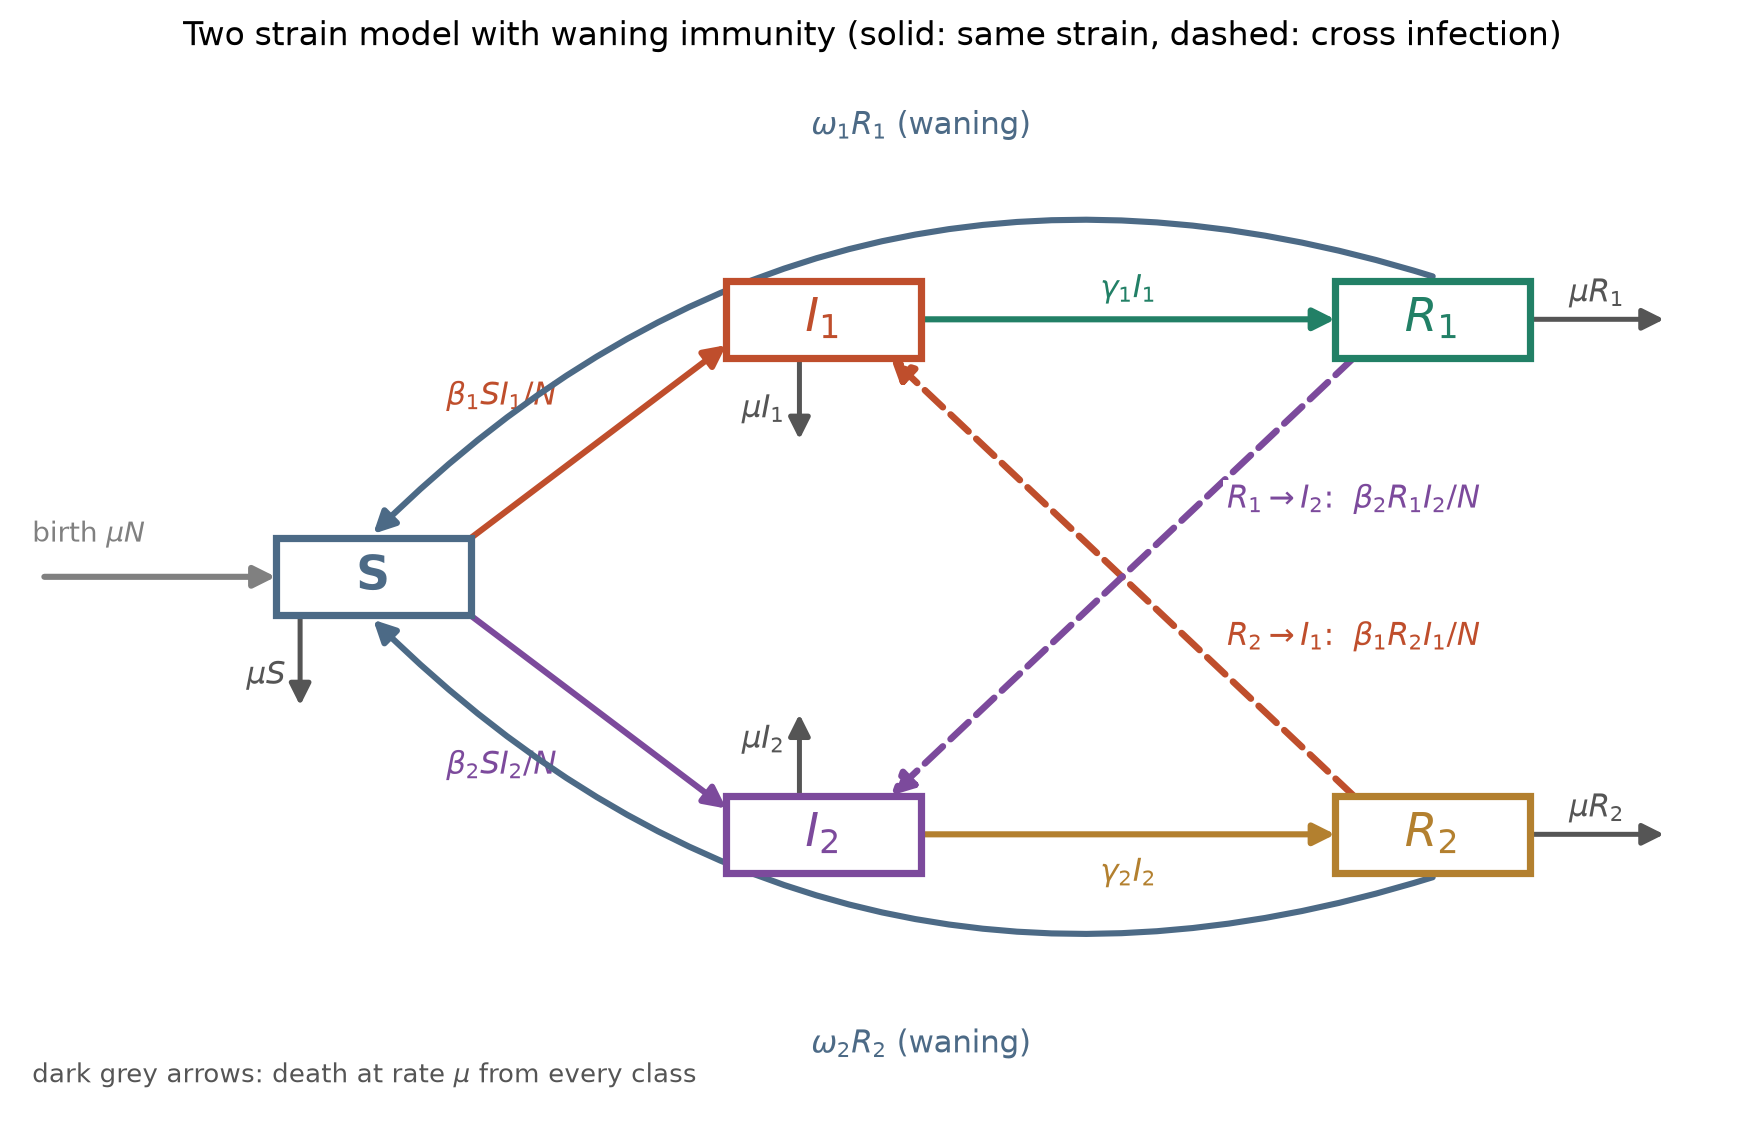
\includegraphics[width=0.82\textwidth]{img/p2fig1.png}
\end{frame}

\begin{frame}{The 14 events (state $[S,I_1,I_2,R_1,R_2]$)}
\small
\renewcommand{\arraystretch}{1.18}
\centering
\begin{tabular}{r l l l}
\rowcolor{aimsred}\color{white}\# & \color{white}Event & \color{white}Change & \color{white}Propensity\\
0 & Birth into $S$ & $[+1,0,0,0,0]$ & $\mu N$\\
\rowcolor{rowpink} 1 to 5 & Death of $S,I_1,I_2,R_1,R_2$ & $-1$ in that class & $\mu S,\mu I_1,\mu I_2,\mu R_1,\mu R_2$\\
6 & $S\to I_1$ & $[-1,+1,0,0,0]$ & $\beta_1SI_1/N$\\
\rowcolor{rowpink} 7 & $S\to I_2$ & $[-1,0,+1,0,0]$ & $\beta_2SI_2/N$\\
8 & $R_2\to I_1$ & $[0,+1,0,0,-1]$ & $\beta_1R_2I_1/N$\\
\rowcolor{rowpink} 9 & $R_1\to I_2$ & $[0,0,+1,-1,0]$ & $\beta_2R_1I_2/N$\\
10 & $I_1\to R_1$ & $[0,-1,0,+1,0]$ & $\gamma_1I_1$\\
\rowcolor{rowpink} 11 & $I_2\to R_2$ & $[0,0,-1,0,+1]$ & $\gamma_2I_2$\\
12 & $R_1\to S$ (waning) & $[+1,0,0,-1,0]$ & $\omega_1R_1$\\
\rowcolor{rowpink} 13 & $R_2\to S$ (waning) & $[+1,0,0,0,-1]$ & $\omega_2R_2$\\
\end{tabular}
\\[0.6em]
{\footnotesize These are the propensities the sheet asks us to complete.}
\end{frame}

\begin{frame}{Investigation 2. Eliminating one variable}
\small
Adding the five equations: $\dfrac{d}{dt}(S+I_1+I_2+R_1+R_2)=\mu\,(1-\text{total})$, so the total stays at 1.\\[0.4em]
Put $S=1-I_1-I_2-R_1-R_2$. The equation for $S$ is redundant and the others become
\[
\begin{aligned}
\dot I_1&=\beta_1(1-I_1-I_2-R_1)I_1-(\gamma_1+\mu)I_1\\
\dot I_2&=\beta_2(1-I_1-I_2-R_2)I_2-(\gamma_2+\mu)I_2\\
\dot R_1&=\gamma_1I_1-\beta_2R_1I_2-(\omega_1+\mu)R_1\\
\dot R_2&=\gamma_2I_2-\beta_1R_2I_1-(\omega_2+\mu)R_2
\end{aligned}
\]
\begin{itemize}\setlength\itemsep{0.3em}
  \item In $\dot I_1$ the cross term $+\beta_1R_2I_1$ cancels the $-R_2$ that comes from $S$. The people susceptible to strain 1 are $S+R_2=1-I_1-I_2-R_1$.
  \item We checked the algebra symbolically (sympy): the difference is zero.
\end{itemize}
\end{frame}

\begin{frame}{Investigation 3. Parameters and basic reproduction numbers}
\renewcommand{\arraystretch}{1.4}
\centering
\begin{tabular}{l c c c c}
\rowcolor{aimsred}\color{white}& \color{white}$\beta$ & \color{white}$\gamma$ & \color{white}$\omega$ & \color{white}$\mathcal R_0=\beta/(\gamma+\mu)$\\
Strain 1 & 120 & 52 (1 week) & 0.2 (5 years) & $\mathbf{2.31}$\\
\rowcolor{rowpink} Strain 2 & 100 & 26 (2 weeks) & 0.5 (2 years) & $\mathbf{3.84}$\\
\end{tabular}
\\[0.8em]
All rates per year. $\mu=0.02$ per year, $N=10{,}000$, initial state $[9900,50,50,0,0]$.
\callout{0.85\textwidth}{Both $\mathcal R_0>1$, and strain 2 has the larger one. Classical theory would let strain 2 win.}
\begin{itemize}
  \item The sheet's SSA function stores every event: about 220,000 per simulated year, so about 6 seconds per year. We checked it on a short run, and used a faster version of the same algorithm for 50 years.
\end{itemize}
\end{frame}

\begin{frame}{Investigation 3. ODE and SSA side by side}
\centering
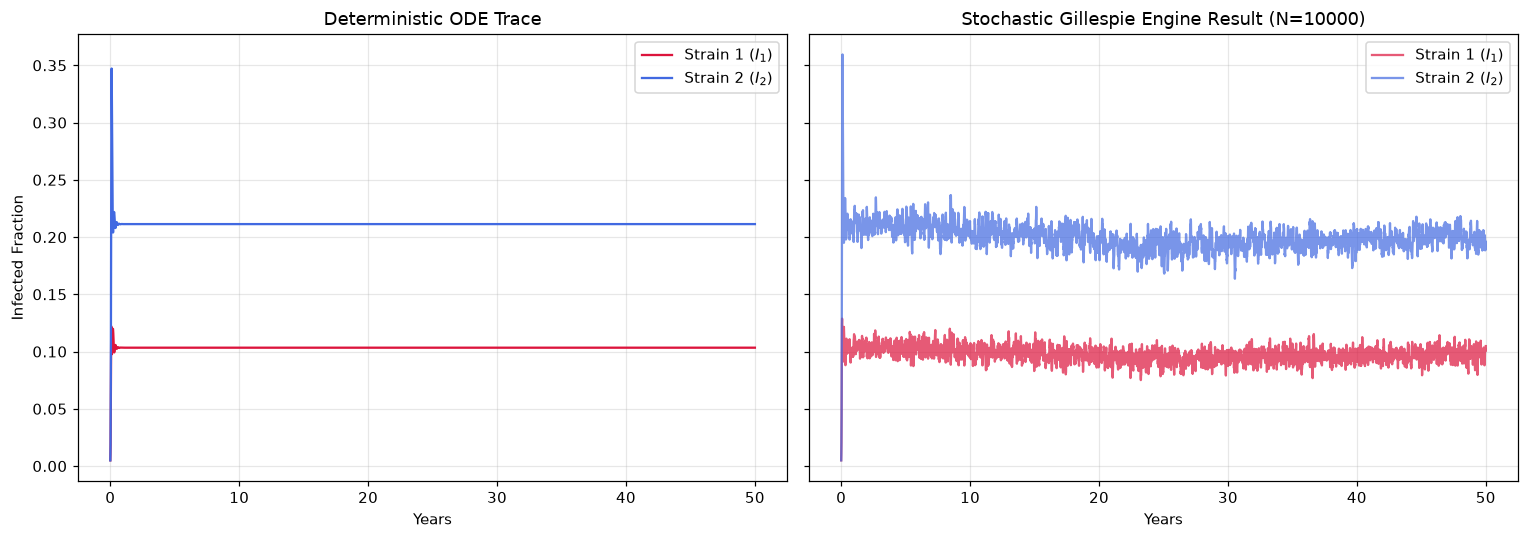
\includegraphics[width=\textwidth]{img/p2fig2.png}
\begin{itemize}\setlength\itemsep{0.3em}
  \item Both strains settle quickly. The SSA fluctuates around the ODE levels (standard deviation about 0.006 and 0.009).
  \item ODE: $I_1^*=0.103$, $I_2^*=0.211$. SSA means over years 10 to 50: 0.096 and 0.197 in this run.
\end{itemize}
\end{frame}

\begin{frame}{Why the SSA level differs a little from the ODE}
\small
\centering
\begin{tabular}{l r r r}
\rowcolor{aimsred}\color{white}Run (20 years) & \color{white}mean total & \color{white}mean $I_1/N$ & \color{white}mean $I_2/N$\\
1 & 10,043 & 0.1046 & 0.2137\\
\rowcolor{rowpink} 2 & 9,905 & 0.0997 & 0.2047\\
3 & 9,966 & 0.1022 & 0.2092\\
\rowcolor{rowpink} 4 & 9,999 & 0.1034 & 0.2114\\
ODE & 10,000 & 0.1034 & 0.2113\\
\end{tabular}
\vspace{0.8em}
\begin{itemize}\setlength\itemsep{0.5em}
  \item In the sheet's SSA, births and deaths are separate random events, so the total population is not fixed. In the 50 year run it ranged from 9,686 to 10,031.
  \item The mean infected level changes by a few percent from run to run (strain 1: 0.096 to 0.105 over five runs, against 0.103). The ODE conserves the total exactly.
  \item The sheet's own SSA code, the fast version and the ODE agree on the mean state after half a year (for example $I_1$: 100.8, 102.5 and 102.4 people at $N=1000$).
\end{itemize}
\end{frame}

\begin{frame}{Investigation 4. Steady coexistence, not cycles}
\begin{columns}[T]
\column{0.52\textwidth}
\begin{itemize}\setlength\itemsep{0.5em}
  \item Overshoot in the first month (peaks near 0.12 and 0.35), then a damped oscillation.
  \item Jacobian eigenvalues: $-8.25\pm33.1i$, $-32.6$, $-18.8$. All negative real parts, so the equilibrium is stable.
  \item Period of the transient about 69 days, half life about one month. No sustained cycles.
\end{itemize}
\column{0.45\textwidth}
\renewcommand{\arraystretch}{1.3}
\begin{tabular}{l r}
\rowcolor{aimsred}\color{white}Class & \color{white}Equilibrium\\
$S^*$ & 0.0084\\
\rowcolor{rowpink} $I_1^*$ & 0.1034\\
$I_2^*$ & 0.2113\\
\rowcolor{rowpink} $R_1^*$ & 0.2518\\
$R_2^*$ & 0.4251\\
\end{tabular}
\end{columns}
\vspace{0.6em}
\callout{0.9\textwidth}{Checked: $S^*+R_2^*=1/\mathcal R_0^1=0.4335$ and $S^*+R_1^*=1/\mathcal R_0^2=0.2602$.}
\end{frame}

\begin{frame}{Why can both strains coexist?}
Strain $i$ alone settles at $S=1/\mathcal R_0^i$. A rare newcomer $j$ faces $S+R_i=1-I_i^*$ susceptible people, so
\[ \mathcal R_{\rm inv}^{\,j\ \mathrm{into}\ i}=\mathcal R_0^{\,j}\,(1-I_i^*). \]
\renewcommand{\arraystretch}{1.35}
\centering
\begin{tabular}{l c c}
\rowcolor{aimsred}\color{white}& \color{white}Strain alone, $I^*$ & \color{white}Invasion number\\
Strain 2 invading strain 1 & $I_1^*=0.0024$ & $3.83>1$\\
\rowcolor{rowpink} Strain 1 invading strain 2 & $I_2^*=0.0145$ & $2.27>1$\\
\end{tabular}
\begin{itemize}\setlength\itemsep{0.4em}
  \item Each strain can invade the other, so neither is excluded.
  \item People recovered from one strain are fresh hosts for the other.
  \item Together they carry far more infection than alone: 43 times more for strain 1 and 15 times more for strain 2.
\end{itemize}
\end{frame}

\begin{frame}{The equations as printed give competitive exclusion}
\centering
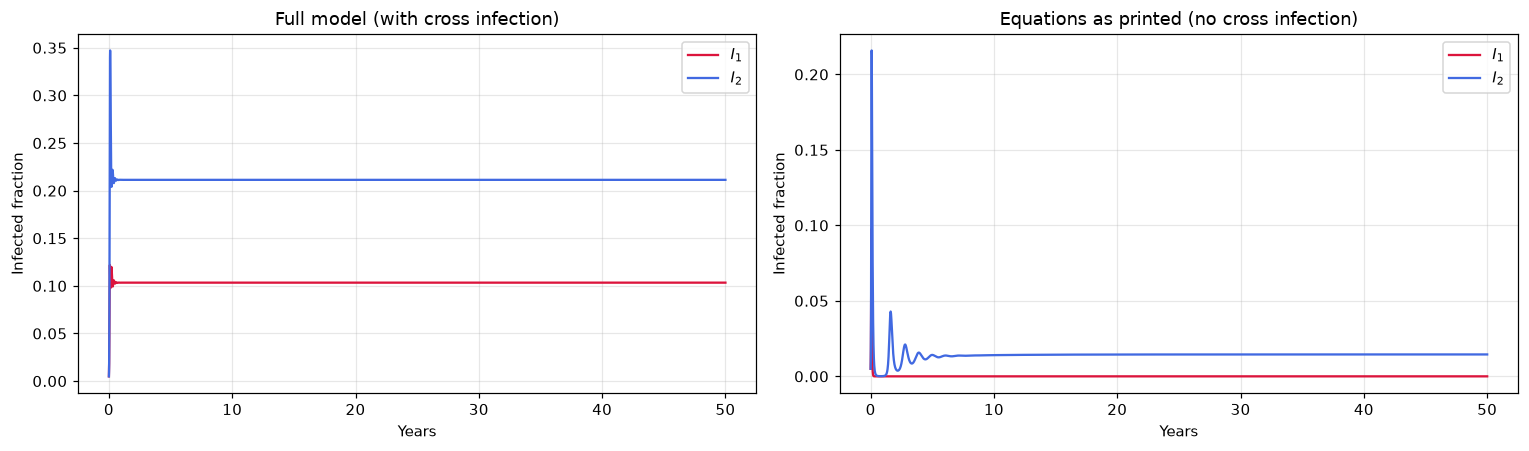
\includegraphics[width=0.95\textwidth]{img/p2fig4.png}
\begin{itemize}\setlength\itemsep{0.3em}
  \item Without cross infection, strain 2 (larger $\mathcal R_0$) wins. At year 50: $I_1\approx10^{-40}$ and $I_2=0.0145$.
  \item So the cross infection is what turns exclusion into coexistence.
\end{itemize}
\end{frame}

\begin{frame}{Stochastic extinction versus deterministic permanence}
\centering
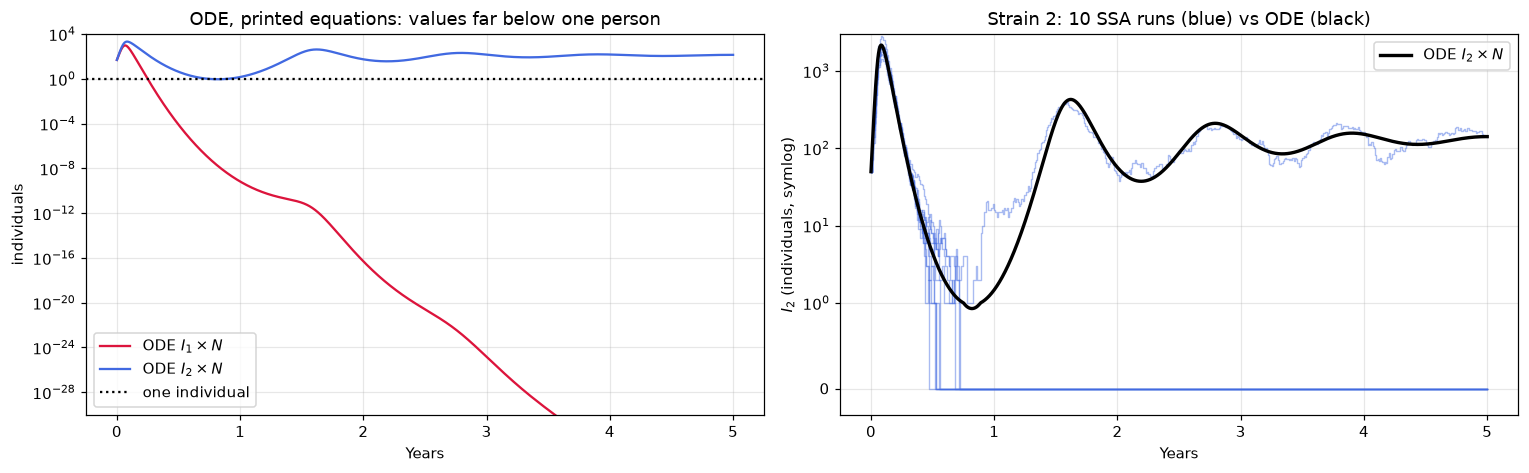
\includegraphics[width=0.95\textwidth]{img/p2fig5.png}
\begin{itemize}\setlength\itemsep{0.3em}
  \item Printed equations. ODE: strain 2 peaks, then dips to 0.93 individuals (year 0.82) and rebounds to 142 individuals by year 5.
  \item SSA, 40 runs: strain 1 lost in 100\% of runs and strain 2 in 85\%. Zero is absorbing, so a lost strain never rebounds.
\end{itemize}
\end{frame}

\begin{frame}{What happens at zero, and why it matters}
\begin{itemize}\setlength\itemsep{0.8em}
  \item \hl{In the SSA:} when $I_i=0$, the infection events of strain $i$ have propensity zero and nothing else creates infection (no immigration). The strain is gone for good.
  \item \hl{In the ODE:} $I_i$ can be tiny and positive and recover later. A fraction $10^{-4}$ of 10,000 people is about one person. $10^{-14}$ is $10^{-10}$ of a person.
  \item \hl{Effect on competition:} a temporary dip in the ODE becomes a permanent loss in the SSA. The survivor is decided by chance as well as by $\mathcal R_0$.
  \item \hl{In the full model at $N=10{,}000$:} no extinction in 50 years, and no crash after the first peak. The ``tiny value then rebound'' picture of the sheet appears for strain 2 in the printed equations, not in the full model.
\end{itemize}
\end{frame}

\begin{frame}{Full model at smaller $N$: extinction appears}
\small
\renewcommand{\arraystretch}{1.3}
\centering
\begin{tabular}{r c c c c c}
\rowcolor{aimsred}\color{white}$N$ & \color{white}start per strain & \color{white}ODE $I_1^*,I_2^*$ (people) & \color{white}P(extinct by yr 50) & \color{white}in year 1 & \color{white}after year 1\\
100 & 1 & 10, 21 & 1.00 & 1.00 & 0.00\\
\rowcolor{rowpink} 200 & 1 & 21, 42 & 1.00 & 0.70 & 0.30\\
400 & 2 & 41, 85 & 0.60 & 0.30 & 0.30\\
\rowcolor{rowpink} 700 & 4 & 72, 148 & 0.08 & 0.08 & 0.00\\
1000 & 5 & 103, 211 & 0.02 & 0.02 & 0.00\\
\end{tabular}
\\[0.4em]
{\footnotesize 40 runs per $N$. Strain 1 and strain 2 have the same extinction fraction in every row: they are lost together.}\\[0.4em]
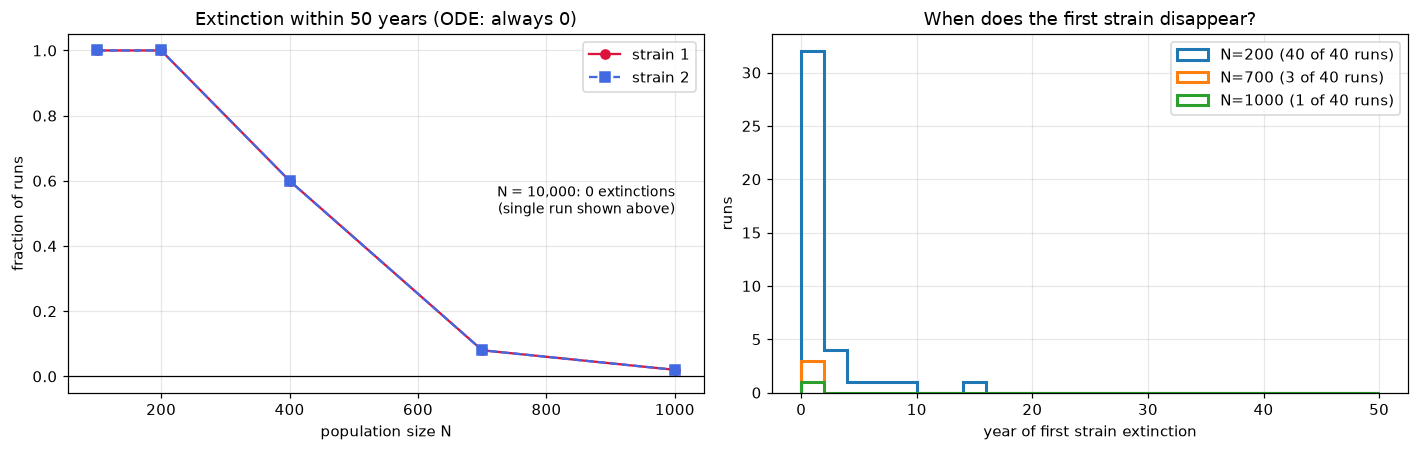
\includegraphics[width=0.78\textwidth]{img/p2fig6.png}
\end{frame}

\begin{frame}{Why the two strains are lost together}
\begin{itemize}\setlength\itemsep{0.8em}
  \item The two strains have the same extinction fraction in every row, and in the example run below they vanish within a quarter of a year of each other.\item Alone, each strain sustains a far smaller infected fraction (0.0024 and 0.0145) than together (0.103 and 0.211).
  \item A likely reason: when one strain disappears, the other is left with very few carriers (for strain 2, about 4 people at $N=300$), and it soon follows. We did not test this mechanism separately.
  \item Coexistence supports itself, and so does collapse.
  \item For $N\ge700$ all extinctions happen in the first year, when only 4 or 5 people carry each strain. For $N\le400$ they also happen later.
\end{itemize}
\centering
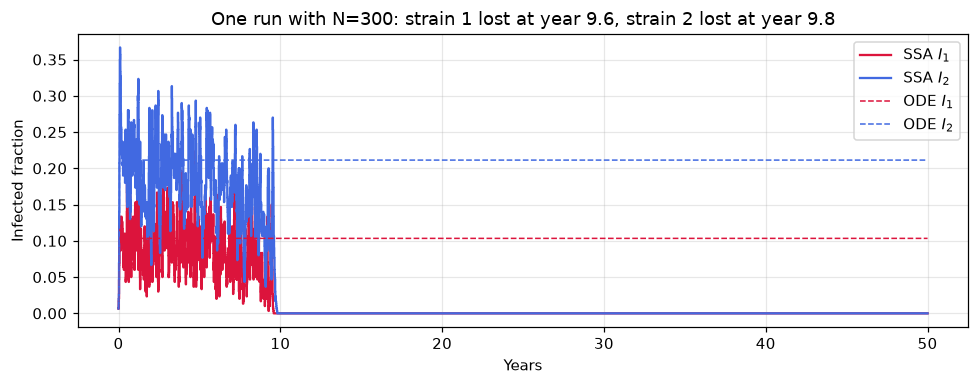
\includegraphics[width=0.62\textwidth]{img/p2fig7.png}
\end{frame}

\begin{frame}{Part 2. Take home message}
\begin{itemize}\setlength\itemsep{0.8em}
  \item With waning immunity and cross infection the ODE gives a \hl{stable coexistence} of both strains, $\mathcal R_0^1=2.31$ and $\mathcal R_0^2=3.84$. No sustained oscillations at these parameters.
  \item Without cross infection (equations as printed) we get classical competitive exclusion.
  \item At $N=10{,}000$ the SSA agrees with the ODE, with fluctuations and a few percent of run to run variation.
  \item At small $N$, or when a strain goes through a bottleneck, the SSA turns tiny ODE values into real extinctions, and extinct strains do not return.
\end{itemize}
\callout{0.9\textwidth}{Deterministic models describe the large population limit. Stochastic models tell us whether a strain actually survives.}
\end{frame}
